\graphicspath{{chapters/19/images}}
\chapter{Rare events}

\section{Introduction}

	\subsection{Rough free energy surfaces}

	\begin{figure}[H]
		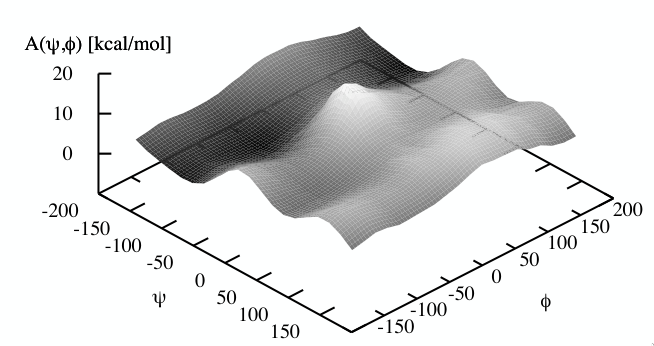
\includegraphics[width=\textwidth]{rough-free-energy-surfaces}
		\caption{Rough free energy surfaces}
		\label{fig:rough-free-energy-surfaces}
	\end{figure}

	\subsection{?????????}

		\begin{itemize}
			\item Reaction coordinates.
			\item Order parameters.
			\item COLVARs.
		\end{itemize}

\section{Reaction coordinates}
Example: $r = |\vec{r}_B-\vec{r}_A|$ for a dissociation reaction $AB\rightarrow A+B$.
Example radius of gyration:

$$R_G = \sqrt{\frac{1}{N_b}\sum\limits_{i=1}^{N_b}\biggl(\vec{r}_i-\frac{1}{N_b}\sum\limits_{j=1}^{N_b}\vec{r}_j\biggr)^2}$$

Example: number of hydrogen bonds of length $d_0$ between $n_O$ oxygens and $n_H$ hydrogens:

$$N_H = \sum\limits_{i=1}^{n_O}\sum\limits_{j=1}^{n_H}\frac{1-\biggl[\frac{\vec{r}_i-\vec{r}_j}{d_0}\biggr]^6}{1-\biggl[\frac{\vec{r}_i-\vec{r}_j}{d_0}\biggr]^{12}}$$

The aim is to obtain the probability distribution function of a subset of $n$ reaction coordinates of interest $q_\alpha= f_\alpha(\vec{r}_1, \dots, \vec{r}_N)$ with $\alpha = 1, \dots, n$:

$$P(s_1, \dots, s_n) = \frac{C_N}{Q(N, V, T)}\int d^N\vec{p}d^B\vec{r}e^{-\beta\mathcal{H}(\vec{r}, \vec{p})}\prod\limits_{\alpha=1}^n\delta(f_\alpha(\vec{r}_1, \dots, \vec{r}_N)-s_\alpha)$$

Free energy hypersurface:

$$A(s_1, \dots, s_n) = -fT\ln P(s_1, \dots, s_n)$$

	\subsection{Blue moon ensemble}
	Single reaction coordinate $q_1 = f_1(\vec{r}_1, \dots, \vec{r}_N)$:

	$$P(s) = \frac{C_N}{Q(N, V, T)}\int d^N\vec{p}d^N\vec{r}e^{-\beta\mathcal{H}(\vec{r}, \vec{p})}\delta(f_1(\vec{r}_1, \dots, \vec{r}_N)-s)$$

	$$A(s) = -kT\ln P(s)$$

	Introduce a holonomic constraint $\sigma(\vec{r}_1, \dots, \vec{r}_N) = f_1(\vec{r}_1, \dots, \vec{r}_N)-s$.
	Use this constraint to drive the reaction coordinate from an initial value $s^{(i)}$ to a final value $s^{(f)}$.
	The blue moon ensemble yields $\frac{dA}{ds} = -\frac{kT}{P(s)}\frac{dP}{ds}$.

	$$A(q) = A(s^{(i)}) + \int_{s^{(i)}}^q\frac{dA}{ds}ds\qquad \Delta A = \int_{s^{(i)}}^{s^{(f)}}\frac{dA}{ds}ds$$

	$$P(s) = \frac{C_N}{Q(N, V, T)}\int d^N\vec{p}d^N\vec{r}e^{-\beta\mathcal{H}(\vec{r}, \vec{p})}\delta(f_1(\vec{r}_1, \dots, \vec{r}_N)-s) = \langle\delta(f_1(\vec{r}_1, \dots, \vec{r}_N)-s)\rangle$$

	$$\frac{1}{P(s)}\frac{dP}{ds} = \frac{C_N}{Q(N, V, T)}\frac{\int d^N\vec{p}d^N\vec{r}e^{-\beta\mathcal{H}(\vec{r}, \vec{p})}\frac{\partial\delta(f_1(\vec{r})-s)}{\partial s}}{\langle\delta(f_1(\vec{r})-s)\rangle}$$

	Introduce $3N$ generalized coordinates $q_\alpha = f_\alpha(\vec{r}_1, \dots, \vec{r}_N)$ and their conjugate momenta $p_\alpha$,
	The transformation is canonical, hence: $d^N\vec{p}d^N\vec{r} = d^{3N}pd^{3N}q$:

	$$\frac{1}{P(s)}\frac{dP}{ds} = \frac{C_N}{Q(N, V, T)}\frac{\int d^{3N}pd^{3N}qe^{-\beta\tilde{\mathcal{H}}(q, p)}\frac{\partial\delta(q_1-s)}{\partial s}}{\langle\delta(q-s)\rangle}$$

	However $\frac{\partial}{\partial s}\delta(q_1-s) = -\frac{\partial}{\partial q_1}\delta(q_1-s)$.
	Integrating by parts:

	\begin{align*}
		\frac{1}{P(s)}\frac{dP}{ds} &=-\frac{\beta C_N}{Q(N, V, T)}\frac{\int d^{3N}pd^{3n}q\frac{\partial\tilde{\mathcal{H}}}{\partial q_1}e^{-\beta\tilde{\mathcal{H}}(q, p)}\delta(q_1-s)}{\langle\delta(q_1-s)\rangle} = \\
																&= -\frac{\beta}{\langle\delta(q_1-s)\rangle}\biggl\langle\frac{\partial\tilde{\mathcal{H}}}{\partial q_1}\delta(q_1-s)\biggr\rangle \equiv -\beta\biggl\langle\frac{\partial\tilde{\mathcal{H}}}{\partial q_1}\biggr\rangle^{cond}
	\end{align*}

	$$A(q) = A(s^{(i)}) + \int_{s^{(i)}}^q\biggl\langle\frac{\partial\tilde{\mathcal{H}}}{\partial q_1}\biggr\rangle^{cond}_sds$$

	\subsection{Umbrella sampling}
	Constraint from the blue moon ensemble are transformed into harmonic restraint into umbrella sampling.

	$$W_k(f_1(\vec{r}_1, \dots, \vec{r}_N), s_k) = \frac{1}{k}[f_1(\vec{r}_1, \dots, \vec{r}_N)-s_k]^2$$

	Biased probability distributions $P(s, s^{(k)}), k= 1, \dots, n,\qquad s^{(1)}=s^{(i)}, s^{(n)}=s^{(f)}$.

	\subsection{WHAM}
	Biased probability distributions generated by umbrella sampling:

	$$\tilde{P}(q, s^{(k)}) = e^{\beta A_k}\int d^N\vec{r}e^{-\beta U(\vec{r})}e^{-\beta W_k(f_1(\vec{r}), s^{(k)})}\delta(f_1(\vec{r})-q)$$

	$A_k$ is the free energy associated with the biasing potential apart from constants:

	$$e^{-\beta A_k} = \int d^N\vec{r}e^{-\beta U(\vec{r})}e^{-\beta W_k(f_1(\vec{r}), s^{(k)})}=e^{-\beta A_0}\biggl\langle e^{-\beta W_k(f_1(\vec{r}), s^{(k)})}\biggr\rangle$$

	The average is taken with respect to the unbiased potential:

	$$e^{-\beta A_0} = \int d^N\vec{r}e^{-\beta U(\vec{r})}$$

	Unbiased probability distributions:

	$$P_k(q) = e^{-\beta(A_k-A_0)\beta W_k(q, s^{(k)})}\tilde{P}(q, s^{(k)})$$

	$\tilde{H}_k(q)$ is the biased histogram obtained from each molecular dynamics or Monte Carlo simulation.
	The estimate for the biased distributions:

	$$\tilde{P}(q, s^{(k)}) \approx\frac{1}{n_k\Delta q}\tilde{H}_k(q)$$

	Statistical error for the umbrella window $\tilde{\sigma}^2_k = \frac{\epsilon_k(q)\tilde{H}_k(q)}{n_k\Delta q}$.
	Error in $P_k(q)$ is given by applying the square of the unbiasing  factor:

	$$\sigma_k^2 = e^{-2\beta(A_k-A_0)}e^{2\beta W_k(q, s^{(k)})}\tilde{\sigma}_k^2$$

	Total error: $\sigma^2 = \sum\limits_{k=1}^nC_k^2(q)\sigma_k^2$.
	Lagrange multiplier: minimize the function:

	$$\Sigma^2=\sum\limits_{k=1}^nC_k^2(q)e^{-2\beta (A_k-A_0)}e^{w\beta W_k(q, s^{(k)})}\frac{\epsilon_k(q)\tilde{H}_k(q)}{n_k\Delta q}-\lambda\biggl(\sum\limits_{k=1}^nC_k(q)-1\biggr)$$

	$$\frac{\partial\Sigma^2}{\partial C_k(q)} = 0\Rightarrow C_k(q) = \frac{\lambda n_k\Delta q}{2\epsilon_k(q)\tilde{H}_k(q)e^{-2\beta(A_k-A_0)}e^{2\beta W_k(q, s^{(k)})}}$$

	Normalization:

	$$\lambda = \frac{1}{\sum\limits_{k=1}^n\frac{n_k\Delta q}{2\epsilon_k(q)\tilde{H}_k(q)e^{-2\beta(A_k-A_0)}e^{2\beta W_k(q, s^{(k)})}}}$$

	$$C_k(q) =\frac{n_kl\bigl[\epsilon_k(q)\tilde{H}_k(q)e^{-2\beta(A_k-A_0)}e^{2\beta W_k(q, s^{(k)})}\bigr]}{\sum\limits_{j=1}^n n_jl\bigl[\epsilon_j(q)\tilde{H}_j(q)e^{-2\beta(A_j-A_0)}e^{2\beta W_k(q, s^{(j)})}\bigr]}$$

	Simplifying assumption:

	\begin{multicols}{2}
		\begin{itemize}
			\item $\epsilon_k(q)$ is the same for all umbrella windows.
			\item $\tilde{H}_k(q)\propto e^{\beta(A_k-A_0)}e^{-\beta W_k(q, s^{(k)})}P(q)$.
		\end{itemize}
	\end{multicols}

	$$C_k(q) = \frac{n_ke^{\beta A_k}e^{-\beta W_k(q, s^{(k)})}}{\sum\limits_{j=1}^nn_je^{\beta A_j}e^{-\beta W_j(q, s^{(j)})}}$$

	$$P(q) = \sum\limits_{k=1}^nC_k(q)P_k(q) = \frac{\sum\limits_{k=1}^nn_k\tilde{P}(q, s^{(k)})}{\sum\limits_{k=1}^nn_ke^{\beta(A_k-A_0)}e^{-\beta W_k(q, s^{(k)})}}$$

	However:

	$$e^{\beta(A_k-A_0)} = \int dq P(q)e^{-\beta W_k(q, s^{(k)})}$$

	Self consistent equations: start with a guess for $A_k$ and iterate until convergence.

	\subsection{Wang-Landau sampling}
	Wang-Landau approach: $A(\vec{r}_2|\vec{r}_1) = \min\biggl[1, \frac{\Omega(E_1)}{\Omega(E_2)}]\biggr]$ with scaling factor $f$.
	Extension to reaction coordinates: generate a function $g(s)$ that approaches the probability distribution $P(s)$.
	Start $g(s)=1$ and $h(s) = \ln g(s) = 0$ everywhere:

	$$A(\vec{r}_2|\vec{r}_1) = \min\biggl[1, \frac{e^{-\beta U(\vec{r}_2)}}{e^{-\beta U(\vec{r}_1)}}\frac{g(s_1)}{g(s_2)}\biggr] = \min\biggl[1, \frac{e^{-\beta U(\vec{r}_2)}}{e^{-\beta U(\vec{r}_1)}}\frac{e^{-h(s_1)}}{e^{-h(s_2)}}\biggr]$$

	$$h(s_2) \rightarrow h(s_2) + \alpha \Leftrightarrow g(s_2)\rightarrow fg(s_2)\qquad \alpha = \ln f$$

	Iterate until the histogram $H(s)$ becomes flat, then reduce $f$ and repeat until convergence.
